\subsection{Übertragung von Daten}

Die Daten müssen auf beiden \ac{uC} ordnungsgemäß empfangen werden. Die Implementation unterscheidet sich hierbei stark. Der STM32 ermöglicht
die Nutzung seiner \ac{DMA}-Funktionalität, während auf dem ESP8266 eine interruptbasierte Abfrage implementiert wird.

\subsubsection{STM32: Strukturvariable DMA\_STRUCT}
\label{subsub: DMASTRUCT}

Aus Gründen der Übersichtlichkeit wurde für die Datenverarbeitung des STM32 eine Strukturvariable definiert, welche hiermit eingeführt wird.
Die Strukturvariable \lstinline!DMA_STRUCT! enthält mehrere weitere Variablen für Flags und Zähler.

\begin{lstlisting}[caption={\textit{DMA Strukturvariable}}]
typedef struct
{
    volatile uint8_t  t_flag;   
    uint8_t tx_flag;	
    volatile uint8_t av_flag;		
    uint16_t timer;             
    uint16_t prevCOUNT;      
    uint8_t data[DMA_BUF_SIZE];   
} DMA_STRUCT;
\end{lstlisting}

Die Flags \lstinline!t_flag! und \lstinline!tx_flag! dienen der Identifikation von Interrupts. Die Interrupts werden im Falle von \lstinline!t_flag! durch ein
Timeout ausgelöst und im Falle von \lstinline!tx_flag! durch das erfolgreiche Senden von Daten. Die Variable \lstinline!timer! legt 
die Zeitkonstante für den Timeout fest, während \lstinline!prevCOUNT! einen Zähler speichert, der in \ref{subsub: Empfang} genauer erklärt wird.  

Das Flag \lstinline!av_flag! zeigt an, wenn neue Daten zur Verarbeitung verfügbar sind. Im Array \lstinline!data[]! werden die neuen Daten gespeichert.

\subsubsection{STM32: Konfiguration des UART}
Wichtig bei der Konfiguration des \acs{UART}, ist das Format und die Baudrate. Wie in Kapitel \ref{sec:Grundlagen} erläutert, wird der \ac{UART} im 8N1-Modus
konfiguriert. Dies entspricht einer Nachrichtenlänge von acht Bit und keiner Parität. Die Geschwindigkeit wird auf 115200 Baud festgelegt (siehe Abb. \ref{img: Parameter}). 

\begin{figure}[h]
  \centering
  \begin{subfigure}{0.45\textwidth}
      \centering
      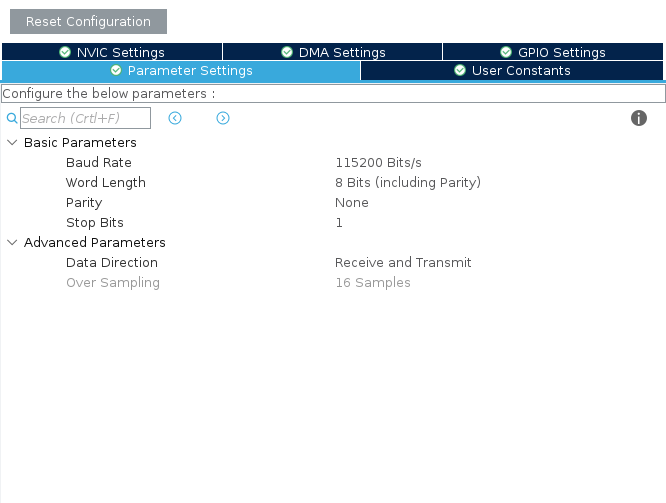
\includegraphics[width=\textwidth]{Pictures/parameter_uart.png}
      \caption{\textit{Baudrate,Format}}
      \label{img: Parameter}
  \end{subfigure}
  %
  \begin{subfigure}{0.45\textwidth}
      \centering
      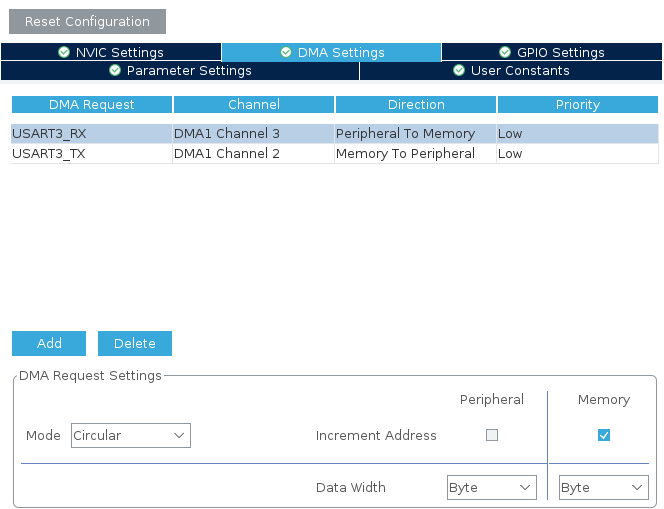
\includegraphics[width=\textwidth]{Pictures/dma_uart.png}
      \caption{\textit{DMA}}
      \label{img: DMA}
  \end{subfigure}
  \caption{\textit{Konfiguration des \acp{UART}}}
  \label{img: UART config}
\end{figure}

Um die Nutzung des \ac{UART} in Kombination mit \ac{DMA} zu ermöglichen, muss der globale Interrupt
aktiviert werden. Der \ac{DMA} wird so konfiguriert, dass empfangsseitig die Daten direkt zum Speicher übertragen werden. Senderseitig werden die Daten
direkt vom Speicher an den \ac{UART} weitergeleitet. Der Empfang von Daten per \ac{DMA} wird durch einen Ringbuffer umgesetzt (siehe Abb. \ref{img: DMA}).


\newpage
\subsubsection{STM32: Idle Line Detection}
  \label{subsub: Idle}
  Eine Idle Line Detection, welche erkennt, wenn keine Daten mehr empfangen werden, wird implementiert. Dies vermeidet das Schreiben von sinnlosen
  Daten in den Buffer, wenn keine Daten mehr empfangen werden.

  \smallskip

  Der STM32 bietet dafür einen Interrupt, welcher manuell aktiviert werden muss \citep{STM32_Ref}:
  \begin{lstlisting}[caption={\textit{Aktivierung Idle Line Interrupt}}]
    __HAL_UART_ENABLE_IT(&huart3,UART_IT_IDLE);
  \end{lstlisting}
  
  Zudem muss in der Datei \lstinline!stm32f1xx_it.c! die Funktion \lstinline!void USARTX_IRQHandler(void)! erweitert werden:

  \begin{lstlisting}[caption={\textit{Idle Line Interrupt Clear}}]
    if(__HAL_UART_GET_FLAG(&huartx,UART_FLAG_IDLE))
    {
        __HAL_UART_CLEAR_IDLEFLAG(&huartx);
        dma_info.timer = DMA_TIMEOUT_MS;
    }
  \end{lstlisting}

  Immer, wenn ein Interrupt in Zusammenhang mit dem \ac{UART} ausgelöst wird, wird die Routine \lstinline!void USARTX_IRQHandler(void)! 
  aufgerufen und geprüft, ob es sich um ein Idle Line Interrupt handelt \citep{STM32_Ref}. 

  \smallskip

  Es ist allerdings nicht ausreichend, nur zu prüfen, ob der Interrupt aufgetreten ist, es kann durchaus vorkommen, dass es sich nur um eine
  kurze Unterbrechung in der Kommunikation handelt. Deshalb wird die Funktionalität um einen Timeout erweitert. Wenn der Interrupt auftritt, wird
  gleichzeitig die Strukturvariable \lstinline!dma_info.timer! mit dem zuvor definierten Zeitwert \lstinline!DMA_TIMEOUT_MS! geladen.

  \smallskip

  Um für zukünftige Erweiterungen keinen Timer zu blockieren, wird für den Timeout der Systick-Timer (\ref{subsub: Timer}) genutzt. Dieser implementiert eine Routine,
  welche im 10ms-Takt aufgerufen wird. Für diese Funktion wird die Routine in der Datei \lstinline!stm32fxx_it.c! um folgenden Code
  erweitert:

  \begin{lstlisting}[caption={\textit{Systick Timer}}]
    if(dma_info.timer == 1)
    {
        dma_info.t_flag = 1;
        HAL_UART_RxCpltCallback(&huartx);
    }
    if(dma_info.timer) 
    { 
        --dma_info.timer; 
    }



  \end{lstlisting}
  
  Mittels dieser Erweiterung wird der Zähler des Timeouts dekrementiert, bis er 1 erreicht. Wenn dies geschieht, wird ein Flag gesetzt
  und die Interruptroutine \lstinline!HAL_UART_RxCpltCallback!
  
  \lstinline!(&huartx)! aufgerufen, in welcher anschließend der aufgetauchte Interrupt mittels des
  gesetzten Flags identifiziert und verarbeitet wird.
  
\subsubsection{STM32: Empfangsinterrupt / DMA Circular Buffer}
  \label{subsub: Empfang}

  Während der Kommunikation mit \ac{UART} werden verschiedene Interrupts ausgelöst werden. Bei der Nutzung von \ac{DMA} werden Interrupts ausgelöst,
  wenn der Buffer halb voll oder ganz voll ist \citep{STM32_Ref}. Des Weiteren wurde der \ac{uC} so konfiguriert, dass auch bei einem Idle Line Interrupt
  die entsprechende Interruptroutine aufgerufen wird \ref{subsub: Idle}.

  \smallskip

  Die Interruptroutinen sind nach der Generation von Code mittels CubeMX in der Datei \lstinline!stm32f1xx_hal.c! als \lstinline!__weak!
  definiert, werden also neu gesetzt sobald sie ohne das Keyword \lstinline!__weak! definiert werden \citep{HAL_Description}. 

  \smallskip

  In \lstinline!main.c! wird die Interruptroutine für den Empfang von Daten per \ac{UART} mit dem Namen 
  \begin{lstlisting}[caption={\textit{Empfangsinterrupt}}]
    void HAL_UART_RxCpltCallback(UART_HandleTypeDef *huart)
  \end{lstlisting}
  initialisiert. 
  
  \smallskip

  Die Variablen \lstinline!pos!, \lstinline!start! und \lstinline!length! werden für den Ringbuffer benötigt. Die Variable \lstinline!currCount! speichert die aktuelle Position des
  Ringbuffers und wird über den Befehl
  
  \begin{lstlisting}[caption={\textit{Position Ringbuffer}}]
    __HAL_DMA_GET_COUNTER(huart->hdmarx)
  \end{lstlisting}
  beschrieben.

  \newpage

  Die Variable \lstinline!start! enthält die Startposition, ab welcher neue Daten im Ringbuffer enthalten sind. In der Variable \lstinline!length!
  ist die Länge der Daten gespeichert. Tritt ein Interrupt auf, weil der Empfangsbuffer voll ist, berechnet sich die Länge der empfangenen 
  Daten simpel durch folgenden Befehl:
  
  \begin{lstlisting}[caption={\textit{Berechnung Länge}}]
    length = DMA_BUF_SIZE - start;
  \end{lstlisting}
  
  Ein Timeout-Interrupt kann ausgelöst werden, nach dem der Buffer voll ist. Um die falsche Verarbeitung von 
  Daten zu verhindern, wird die aktuelle Position des Buffers auf die Größe des Buffers gesetzt.
  
  \begin{lstlisting}[caption={\textit{Setzen des Zählers bei Timeout}}]
    dma_info.prevCOUNT = DMA_BUF_SIZE;      
  \end{lstlisting}

  
  Wird ein Timeout-Interrupt ausgelöst, wird die Routine durch folgenden Code frühzeitig abgebrochen und das Flag zurückgesetzt:
  
  \begin{lstlisting}[caption={\textit{Abbruch Timeoutinterrupt}}]
    if(dma_info.t_flag && currCOUNT == DMA_BUF_SIZE)
    {
        dma_info.t_flag = 0;
        return;
    }
  \end{lstlisting}

  \smallskip

  Tritt ein Interrupt auf, weil ein Timeout stattgefunden hat, muss unterschieden, werden ob im Buffer bereits alte Daten liegen, welche ignoriert
  werden müssen oder ob der Buffer mit zu verarbeitenden Daten gefüllt ist. Dies wird durch folgenden Code implementiert:

  \begin{lstlisting}[caption={\textit{Längenberechnung Timeout}}]
    if(dma_info.t_flag)
    {
    	if(dma_info.prevCOUNT < DMA_BUF_SIZE)
    	{
    		length = dma_info.prevCOUNT - currCOUNT;
    	}
    	else
    	{
  		length = DMA_BUF_SIZE - currCOUNT;
  	}

        dma_info.prevCOUNT = currCOUNT;
        dma_info.t_flag = 0;
    }
  \end{lstlisting}

  Tritt ein Timeout-Flag auf, wird geprüft, ob der alte Zähler des Ringbuffers kleiner als die Buffergröße ist. Ist dies der Fall, berechnet
  sich die Länge der Daten durch die Differenz zwischen dem alten und dem neuen Zählerwert, da alte Daten im Buffer gespeichert sind.
  
  Wenn keine alten Daten im Buffer gespeichert sind, berechnet sich die Länge durch die Differenz zwischen der Buffergröße und der aktuellen Zählerposition.

  \smallskip

  Im Anschluss wird der Zählerwert des \ac{DMA} übergeben und das Timeout-Flag auf 0 zurückgesetzt.

  \smallskip

  Die Startposition der neuen Daten berechnet sich ähnlich. Ist der alte Zähler des Ringbuffers kleiner als die Buffergröße, ist die Startposition
  die Differenz zwischen der Buffergröße und des alten Zählerwerts. Wenn nicht, ist die Startposition gleich 0.

  \begin{lstlisting}[caption={\textit{Berechnung Startposition}}]
    if(dma_info.prevCOUNT<DMA_BUF_SIZE)
    {
    	start = (DMA_BUF_SIZE-dma_info.prevCOUNT);
    }
    else
    {
    	start = 0;
    }  
  \end{lstlisting}

  \smallskip

  Mit Hilfe der berechneten Werte für die Startposition und der Länge der empfangenen Daten werden diese Daten in ein dediziertes
  Array zur Weiterverarbeitung kopiert. Außerdem wird ein Flag gesetzt, welches anzeigt, dass neue Daten vorhanden sind:
  
  \begin{lstlisting}[caption={\textit{Kopieren neuer Daten}}]
    for(uint16_t i=0,pos=start; i<length; ++i,++pos)
    {
        dma_info.data[i] = dma_rx_buf[pos];
    }
    dma_info.av_flag = 1;
  \end{lstlisting}

  Die Telegramme lassen sich mit den Informationen über das Protokoll aus \ref{subsub: Datenformat}, aus dem Array in dem die angekommenen
  Daten gespeichert wurden, extrahieren.

\subsubsection{STM32: Überprüfen der Daten}
\label{subsub: data_check}

Die empfangenen Daten müssen auf ihre Integrität getestet werden. Dazu wurde in \ref{subsub: CRC16} das Konzept der zyklischen Redundanzprüfung eingeführt.

\smallskip

Um die empfangenen Daten zu prüfen, wird das Array, welches die Daten enthält, der Funktion \lstinline!uint8_t data_check(uint8_t *dat)!
übergeben. Diese Funktion extrahiert die CRC-Prüfsumme sowie die Länge der Nachricht und validiert diese. Wenn die zyklische 

Redundanzprüfung erfolgreich ist, wird die Länge der Nachricht übergeben. Wenn sie fehlschlägt, wird eine 0 zurückgegeben.

\newpage
\subsubsection{STM32: Verarbeitung der empfangenen Daten}
Wird durch das Flag \lstinline!av_flag! der Strukturvariable \lstinline!DMA_STRUCT! (siehe \ref{subsub: DMASTRUCT}) angezeigt, dass neue Daten
verfügbar sind, werden diese in der Main-Schleife verarbeitet. Mit Hilfe der Funktion \lstinline!data_check()! aus \ref{subsub: data_check}
wird das empfangene Telegramm geprüft und die Länge der Nachricht in der globalen Variable \lstinline!uint8_t data_len! gesichert sowie das Flag
auf 0 zurückgesetzt.

\begin{lstlisting}[caption={\textit{Datenverarbeitung}}]
  if(dma_info.av_flag == 1)
  {
    dma_info.av_flag = 0;
    data_len = data_check(dma_info.data);
\end{lstlisting}

Ist die Länge ungleich 0, war die Prüfung erfolgreich. Mittels eines Switch-Cases wird anschließend geprüft, um welche Art Nachricht
es sich handelt (Nachrichtentypen siehe \ref{subsub: Nachricht}). Es folgt ein Beispiel für die Nachricht STATUS.

\begin{lstlisting}[caption={\textit{Switch Case}}]
  if (data_len != 0) {
    switch (dma_info.data[3]) {

    case STATUS:
      TxLen = ack_send(STATUS, TxBuffer);
      HAL_UART_Transmit_DMA(&huart3, TxBuffer, TxLen);
      tx_wait(&dma_info);

      TxLen = stat_send(TxBuffer);
      HAL_UART_Transmit_DMA(&huart3, TxBuffer, TxLen);
      tx_wait(&dma_info);
      break;
\end{lstlisting}

Wenn die Länge ungleich 0 ist, wird die vierte Stelle des Arrays, welches das Telegramm enthält, geprüft, um den Nachrichtentyp zu bestimmen.
Anschließend wird ein Acknowledge-Telegramm versendet, um den Empfang zu bestätigen. Dies geschieht mittels 
der Funktion \lstinline!ack_send()!. Der Aufbau dieser Funktion ist ähnlich der in \ref{subsub: STM_Telegramm}
erklärten Funktion. Auf den Versandprozess wird in \ref{subsub: VersendenDat} genauer eingegangen. 

\smallskip

Nachdem das Acknowledge-Telegramm verschickt wurde, wird das eigentliche Antworttelegramm versendet (Funktion \lstinline!stat_send()!)
und der Switch-Case beendet.

\smallskip

Ist der Nachrichtentyp keiner bekannten Nachricht zuzuordnen, wird mittels des Default-Cases eine Errornachricht versandt.

\subsubsection{STM32: Erstellen von Telegrammen}
\label{subsub: STM_Telegramm}

Es werden verschiedene Telegramme, abhängig von der Nachricht, versendet. Die Telegramme enthalten neben der eigentlichen Nachricht auch immer eine CRC-Prüfsumme,
Längeninformationen und ein Startzeichen (siehe \ref{subsub: Datenformat}). Um dies zu ermöglichen, wurden diverse Funktionen zum Erstellen von Telegrammen entwickelt.
Dieser Sachverhalt wird an Hand einer Funktion, welche die Antwort auf den Befehl STATUS erstellt, dargestellt. Andere Funktionen, welche z.B. die Messwerte des Sensors
oder eine Empfangsbestätigung versenden, sind ähnlich aufgebaut und unterscheiden sich nur durch den eigentlichen Nachrichteninhalt.

\smallskip

Allen Funktionen wird ein Zeiger auf ein Array übergeben, in welches die Daten geschrieben werden. Zudem geben die Funktionen die Länge des Telegramms zurück.

\smallskip

Die Funktion \lstinline!uint8_t stat_send(uint8_t * txbuf)! schreibt Informationen über den Softwarestand, den genutzten Sensor und die Boardversion in das Array. Diese
Daten sind durch die Defines \lstinline!BOARD!,\lstinline!VERSION! und \lstinline!SENSOR! festgelegt.

\begin{lstlisting}[caption={\textit{Status-Telegramm}}]
  uint8_t stat_send(uint8_t * txbuf)
  {
    uint16_t crc_value;
    
    txbuf[0] = START; 
    txbuf[1] = 0 + OFF_ASCII;
    txbuf[2] = 3 + OFF_ASCII;
    txbuf[3] = BOARD;
    txbuf[4] = VERSION;
    txbuf[5] = SENSOR;
    crc_value = CRC16_buf(txbuf,6);
    txbuf[6] = (crc_value >> 8) & 0xFF;				
    txbuf[7] = (crc_value >> 0) & 0xFF;
  
    return 8;										
  }
\end{lstlisting}

Die Längeninformation wird als \ac{ASCII}-Zahl dargestellt, sie muss deshalb um den entsprechenden Offset (48) verschoben werden. Da die CRC16-Prüfsumme 16 Bit lang ist,
muss diese in zwei jeweils 8 Bit lange Teile aufgeteilt werden. Dies geschieht durch entsprechendes Verschieben nach rechts und der logischen UND-Operation mit der Zahl 
0xFF.

\smallskip

Da das gesamte Telegramm acht Zeichen lang ist, wird eine 8 zurückgegeben.



\subsubsection{STM32: Versenden von Daten}
\label{subsub: VersendenDat}

Das Versenden von Daten geschieht mittels folgender Funktion \citep{HAL_Description}:
\begin{lstlisting}[caption={\textit{Sendefunktion}}]
  HAL_StatusTypeDef HAL_UART_Transmit_DMA(UART_HandleTypeDef *huart,
  uint8_t *pData, uint16_t Size)
\end{lstlisting}

Der Handler, welcher dem genutzten \ac{UART} zugeordnet ist, der zu übertragende Buffer und die Länge des Buffers werden übergeben. 

\smallskip

Wichtig bei der Nutzung der Funktion ist das Abwarten, ob die Daten versendet wurden. Wird die Funktion zu früh ein zweites Mal aufgerufen, werden die Daten,
die sich gerade im Sendebuffer befinden, überschrieben \citep{HAL_Description}. Eine Prüfung, ob die Funktion \lstinline!HAL_OK! zurückgibt, ist nicht ausreichend,
da dies bereits geschieht, bevor alle Daten übertragen wurden.

\smallskip

Ähnlich wie bei dem Empfang von Daten gibt es auch beim Versenden von Daten einen Interrupt, sobald die Daten erfolgreich versendet wurden \citep{HAL_Description}. Mittels des
Flags \lstinline!uart_info.tx_flag!, welches innerhalb der zugehörigen Interruptroutine gesetzt wird, wird die Vollendung der Übertragung kontrolliert.

\smallskip

Dieser Zusammenhang wird in folgender Funktion umgesetzt:

\begin{lstlisting}[caption={\textit{Warten auf Versand}}]
  void tx_wait(DMA_STRUCT * dma)
  {
    while(!dma->tx_flag);						
    dma->tx_flag=0;								
  }
\end{lstlisting}

Es wird die DMA-Strukturvariable übergeben und gewartet, bis das Flag in der Interruptroutine gesetzt wurde. Sobald dies geschehen ist, wird es zurückgesetzt;
neue Daten können versendet werden.



\subsubsection{ESP8266: Empfang und Überprüfung der Daten}
\label{subsub:Empfang8266}

Die Implementation für den Empfang von Daten ist auf Grund des Arduino-Frameworks \citep{ArduinoRef} anders aufgebaut. Die Funktion \lstinline!void receive()!
implementiert die Funktionalität des Datenempfangs. Ähnlich wie bei der Implementation des STM32 wird hier ein Timeout genutzt, jedoch auf \ac{DMA} verzichtet.

\smallskip

Folgende Variablen werden innerhalb der Funktion genutzt:

\begin{lstlisting}[caption={\textit{Variablen receive()}}]
  static uint16_t count = 0;
  static bool InProg = false;
  static uint8_t len= 0;
  uint16_t crc_calc;
  static uint32_t tim;  
\end{lstlisting}

Die Variable \lstinline!count! zählt die Anzahl der empfangenen Bytes, während \lstinline!InProg! anzeigt, dass zurzeit Daten empfangen werden. Zudem speichert
\lstinline!len! die Länge der empfangenen Nachricht, während \lstinline!tim! die Zählervariable für den Timeout implementiert. Um das Ergebnis der zyklischen
Redundanzprüfung zu speichern, wird \lstinline!crc_calc! genutzt.

\smallskip

Zudem werden die globalen Variablen \lstinline!receivedChars[BUF_SIZE]! und \lstinline!newData! benötigt.
Das Array speichert die empfangenen Daten, während durch das Flag \lstinline!newData! die Verfügbarkeit von neuen Daten angezeigt wird.

\smallskip

Die Implementation bedient sich diverser Befehle aus dem Arduino-Framework \citep{ArduinoRef}:

\begin{itemize}
  \item \lstinline!Serial.available()! - Prüfen ob neue Daten vorhanden sind
  \item \lstinline!Serial.read()! - Einlesen eines Bytes 
  \item \lstinline!millis()! - Auslesen der verstrichenen Zeit in ms
\end{itemize}

Um Funktionen, die im Zusammenhang mit dem \ac{UART} stehen, nutzen zu können, muss dieser während des Starts des \ac{uC} mit der Baudrate initialisiert werden \citep{ArduinoRef}:
\begin{lstlisting}[caption={\textit{Konstruktor UART}}]
  Serial.begin(BAUD);
\end{lstlisting}

Die Funktion \lstinline!void receive()! wird kontinuierlich in der Main-Loop aufgerufen.

\smallskip


Mittels einer While-Schleife wird geprüft, ob Daten verfügbar sind und ob Daten, welche zuvor empfangen wurden, verarbeitet werden müssen. Wenn diese Bedingung erfüllt
ist, wird der Zähler des Timers auf den aktuellen Wert aktualisiert und ein Byte eingelesen. 

\begin{lstlisting}[caption={\textit{Prüfen auf neue Daten}}]
  while (Serial.available() > 0 && newData == false)
  {
      tim = millis();
      receivedChars[count] = Serial.read();
\end{lstlisting}

Nach jedem Durchlauf der kompletten While-Schleife wird der Zähler \lstinline!count! inkrementiert, um das nächste Zeichen einzulesen.

\smallskip

Wird ein Start-Zeichen im empfangenen Telegramm (siehe \ref{subsub: Datenformat}) erkannt, wird die Variable \lstinline!InProg! gesetzt, um die weitere Verarbeitung
zu erlauben:

\begin{lstlisting}[caption={\textit{Erkennung Start-Marker}}]
  if (receivedChars[count] == START_MARKER)
  {
    InProg = true;
  }
\end{lstlisting}

Auf Basis der aktuellen Anzahl an eingelesenen Zeichen und dem gesetzten Flag wird nun das Einlesen der Längeninformation ermöglicht:

\begin{lstlisting}[caption={\textit{Einlesen Längeninformation}}]
  if(InProg == true && count == 2)
  {
    len = (receivedChars[count]-OFF_ASCII)
    +((receivedChars[count-1]-OFF_ASCII)*10);
  }
\end{lstlisting}

Die Länge muss dafür zu einer Integervariablen konvertiert werden. Dies geschieht durch die Subtraktion des Offsets (48) und das Zusammenführen der verschiedenen Stellen.

\smallskip

Basierend auf der eingelesenen Länge der Nachricht kann festgestellt werden, wann die CRC-Prüfsumme eingelesen wurde (siehe \ref{subsub: Datenformat}). Mittels der Prüfsumme
wird dann die zyklische Redundanzprüfung durchgeführt. Bei Erfolg werden die Variablen der Funktion zurückgesetzt sowie das Flag zum Anzeigen von neuen Daten gesetzt. War die Prüfung
nicht erfolgreich, wird das Flag nicht gesetzt.

\begin{lstlisting}[caption={\textit{Zyklische Redundanzprüfung}}]
  if(InProg == true && count == len+4){
        crc_calc = CRC16_buf(receivedChars,count+1); 
        if(crc_calc == 0)
        {
          length_pub = len;
          InProg = false; 
          newData = true; 
          len = 0;        
          count = 0;      
          return;
        }
        else{
          InProg = false;  
          newData = false; 
          len = 0;         
          count = 0;        
          return;         
        }
\end{lstlisting}

Da der Zähler \lstinline!count! am Ende der While-Schleife inkrementiert wird, muss der Funktion der zyklischen Redundanzprüfung \lstinline!count+1! übergeben werden.

\smallskip

Bevor jedoch die soeben erklärte While-Schleife aufgerufen wird, muss geprüft werden, ob ein Timeout eingetreten ist. Diese Überprüfung bedient sich der gespeicherten Zeit,
der aktuellen Zeit sowie dem Flag \lstinline!InProg!, welches anzeigt, ob eine Transaktion läuft. Ist die Differenz zwischen aktueller Zeit und der gespeicherten Zeit
größer als das definierte Timeout und das Flag gesetzt, werden die Variablen \lstinline!count! und \lstinline!InProg! zurückgesetzt und das Einlesen abgebrochen:

\begin{lstlisting}[caption={\textit{Abbruch durch Timeout}}]
  if (InProg == true && (millis() - tim > TIMEOUT))
  {
    count = 0;
    InProg = false;
  }
\end{lstlisting}

\subsubsection{ESP8266: Anmelden an WLAN und MQTT-Server}
\label{subsub: AnmeldenMQTT}

Um die Datenübertragung per \ac{MQTT} an ein übergeordnetes Netzwerk zu ermöglichen, wird eine drahtlose Netzwerkverbindung per \acs{WLAN}
eingesetzt. Hierfür ist es notwendig, den ESP8266 beim Netzwerk anzumelden. Dies geschieht mittels der ESP8266-WiFi Library \citep{ESPWiFi}.
Sobald die Verbindung erfolgreich hergestellt ist, meldet sich der ESP8266 beim \ac{MQTT}-Server an, welcher sich im selben Netzwerk befindet.

\smallskip

Das Anmelden am \acs{WLAN} erfolgt über die
Funktion \lstinline!void setup_wifi()!, diese enthält die Logik zum Aufbau der Verbindung. Es muss jedoch während der Variablendeklaration der
Konstruktor aufgerufen werden, um die enstprechende Klasse zu initialisieren:
\begin{lstlisting}[caption={\textit{Konstrukor WLAN-Library}}]
  WiFiClient espClient;
\end{lstlisting}


\smallskip

Um den Verbindungsaufbau zu signalisieren, leuchtet, während die Verbindung aufgebaut wird, die auf der Platine angebrachte LED auf. 
Die globalen Variablen \lstinline!ssid! und \lstinline!password! speichern den Namen und das Kennwort des drahtlosen Netzwerkes, 
mit welchem die Verbindung hergestellt wird.
\begin{lstlisting}[caption={\textit{Anmelden an \acs{WLAN}}}]
  void setup_wifi() {
  bool led_flag = 0;
  delay(10);
  WiFi.begin(ssid, password);
  while (WiFi.status() != WL_CONNECTED) {
    delay(500);
    if (led_flag==0)
    {
      digitalWrite(ledPin,HIGH);
      led_flag = 1;
    }
    else
    {
      digitalWrite(ledPin,LOW);
      led_flag = 0;
    }
  }
  digitalWrite(ledPin,LOW);
}
\end{lstlisting}

Die Funktion \lstinline!WiFi.begin! initiert die Verbindung mit den Anmeldedaten des Netzwerkes. Solange die Verbindung nicht aufgebaut wurde, signalisiert
durch \lstinline!WL_CONNECTED!, blinkt die LED alle 0.5s auf. Sobald die Verbindung erfolgreich hergestellt wurde, wird die LED abgeschaltet.

\newpage

Die Verbindung zum \acs{MQTT}-Server wird hergestellt,
wenn die Verbindung zum \ac{WLAN} erfolgreich hergestellt wurde. Der Server muss sich im selben Netzwerk befinden. Der Server wird mittels eines
RaspberryPis realisiert (siehe \ref{subsub: MQTT_RasPi}). 

\smallskip

Um die Kommunikation per \ac{MQTT} zu vereinfachen, wird auf die Library PubSubClient \citep{PubSub} zurückgegriffen. Die IP des \ac{MQTT}-Servers
wird in der globalen Variable \lstinline!mqtt_server! gespeichert. Die Funktion \lstinline!void reconnect()! übernimmt den Verbindungsaufbau.
Um Daten per \ac{MQTT} zu empfangen, wird ein Callback implementiert, eine Funktion, welche bei Empfang von Daten aufgerufen wird:

\begin{lstlisting}[caption={\textit{MQTT Callback}}]
  void callback(String topic, byte* message, unsigned int length)
\end{lstlisting}

Die Variablen der Funktion enthalten Informationen über die Länge der Nachricht, das Topic, unter welchem die Nachricht empfangen wurde, 
sowie den eigentlichen Nachrichteninhalt.

\smallskip

Während der Variablendeklaration wird der Konstruktor der Bibliothek aufgerufen, welcher die Informationen über die \ac{WLAN}-Verbindung
übernimmt:

\begin{lstlisting}[caption={\textit{MQTT Konstruktor}}]
  PubSubClient client(espClient);
\end{lstlisting}

Während der Initialiserung, nachdem die Verbindung zum \ac{WLAN}-Netzwerk hergestellt wurde, werden die Verbindungsinformationen des 
\ac{MQTT}-Servers gespeichert und der Callback gesetzt:


\begin{lstlisting}[caption={\textit{MQTT Initialisierung}}]
  setup_wifi();
  client.setServer(mqtt_server,1883);
  client.setCallback(callback);
\end{lstlisting}

Innerhalb der Main-Schleife wird fortlaufend geprüft, ob die Verbindung besteht. Wenn dies nicht der Fall ist, wird diese mittels der Funktion
\lstinline!reconnect()! wiederhergestellt. Mit der Funktion \lstinline!client.loop()! wird geprüft, ob neue Daten per \ac{MQTT} empfangen wurden
und gegebenenfalls der Callback aufgerufen.
\begin{lstlisting}[caption={\textit{MQTT Verbindungsprüfung, Datenempfang}}]
  if (!client.connected()) {
    reconnect();
  }
  client.loop(); 
\end{lstlisting}

Die Funktion \lstinline!void reconnect()! implementiert den Verbindungsaufbau zum \ac{MQTT}-Server. Dem Client (in diesem Falle der ESP8266)
muss ein einzigartiger Name zur Identifikation vergeben werden. Wenn ein anderes Gerät denselben Namen besitzt, kommt es zu Fehlern. Dieser
Name wird in der Variable \lstinline!clientId! gespeichert. 

\smallskip

Während die Verbindung aufgebaut wird, leuchtet die LED auf der Platine, um den Prozess anzuzeigen. Wurde die Verbindung erfolgreich aufgebaut,
wird eine Nachricht (\glq Sensor connected! \grq) geteilt und das Topic, auf welchem in Zukunft Befehle empfangen werden sollen, abonniert. Anschließend wird die LED
abgeschaltet.

\begin{lstlisting}[caption={\textit{Funktion reconnect()}}]
  void reconnect() 
  {
    while (!client.connected()) 
    {
      if (client.connect(clientId.c_str())) 
      {
        client.publish("Humid", "Sensor connected!");
        client.subscribe("SensorSetup");
        digitalWrite(ledPin,LOW);
      } else 
      {
        digitalWrite(ledPin,HIGH);
        delay(5000);
      }
    }
  }    
\end{lstlisting}

\subsubsection{ESP8266: Empfang und Versand per MQTT}

Der Versand von Nachrichten geschieht durch die Funktion \lstinline!client.publish()!. Ihr werden das Topic, die Daten, welche übertragen
werden sollen (in Form eines Arrays) sowie die Länge des Arrays übergeben. Die Funktion wird innerhalb der Main-Schleife immer dann
aufgerufen, wenn durch das Flag \lstinline!newData! angezeigt wird, dass neue Daten verfügbar sind (siehe \ref{subsub:Empfang8266}).

\smallskip

Es ist dabei zu beachten, dass die Startzeichen sowie die Längenangabe nicht übertragen werden sollen, sondern nur der Nachrichteninhalt.
Dies erklärt den Offset +3 des Arrays. Das Flag \lstinline!newData! muss zurückgesetzt werden, um ein erneutes Versenden zu ermöglichen.

\begin{lstlisting}[caption={\textit{Versand per MQTT}}]
  if (newData == true)
  {
    client.publish("Humid",receivedChars+3,length_pub);  
    newData = false;
  }
\end{lstlisting}

Der Empfang von Daten geschieht mittels des in \ref{subsub: AnmeldenMQTT} erwähnten Callbacks. Dieser wird aufgerufen, sobald neue Daten
verfügbar sind. In dieser Routine werden die Daten direkt per \ac{UART} an den STM32 weitergereicht. Dem Callback werden Variablen
übergeben, die das Topic und die Länge der Nachricht enthalten, sowie ein Zeiger auf das Array mit der eigentlichen Nachricht.

\smallskip

Die Variable \lstinline!uint16_t crc16! dient der Speicherung der berechneten CRC-Prüfsumme. Das Array \lstinline!char len_buf[2]! speichert
die Längenangabe der empfangenen Nachricht. Dem Callback wird die Längenangabe als Integervariable übergeben, darum ist eine Konversion
zu einem Char-Array notwendig, da die Kommunikation unter Nutzung des \ac{ASCII}-Standards geschieht. Das globale Array 
\lstinline!uint8_t mqtt_in_data! speichert die Daten, welche empfangen wurden, inkl. der hinzugefügten Startmarker, Längeninformationen etc.

\begin{lstlisting}[caption={\textit{Längenkonversion}}]
  void callback(String topic, byte* message, unsigned int length) {
  char len_buf[2];
  uint16_t crc16;

  sprintf(len_buf,"%d",length); 

  mqtt_in_data[0]=START_MARKER; 

  if (length <10){
    mqtt_in_data[1] = '0';
    mqtt_in_data[2] = len_buf[0];
  }
  else{
    mqtt_in_data[1] = len_buf[0];
    mqtt_in_data[2] = len_buf[1];
  }
\end{lstlisting}

Die Funktion \lstinline!sprintf()! ermöglicht die Konversion einer Integervariablen zu einem Char-Array unter Angabe der Länge \lstinline!length!.
Es muss allerdings darauf geachtet werden, dass unter Nutzung des in \ref{subsub: Datenformat} erklärten Formates bei einer Länge <10
das erste Byte der Längeninformation 0 sein muss und in diesem Falle die Länge in \lstinline!len_buf[0]! gespeichert wird.

Ist die Länge >10, wird in \lstinline!len_buf[0]! die Einerstelle und in \lstinline!len_buf[1]! die Zehnerstelle gespeichert. Desweiteren wird, 
dem Protkoll entsprechend, der erste Wert des Arrays mit dem Startmarker beschrieben.

\smallskip

Die eigentliche Nachricht wird anschließend dem Ausgabearray übergeben und die CRC-Prüfsumme berechnet. Der Länge \lstinline!length!
muss dabei die Anzahl der hinzugefügten Bytes addiert werden (+3). Anschließend wird die 16-Bit breite Prüfsumme geteilt und angehängt.


Um das Telegramm im Anschluss an den STM32 auszugeben wird das Array \lstinline!mqtt_in_data[]! mit Hilfe der Arduino-Funktion \lstinline!Serial.print()!
per \ac{UART} versendet.

\newpage

\begin{lstlisting}[caption={\textit{Ausgabe MQTT-Nachricht}}]
  for (uint8_t i = 0; i < length; i++)   
  {
    mqtt_in_data[i+3] = message[i];
  }

  crc16 = CRC16_buf(mqtt_in_data,length+3); //calc the crc16

  mqtt_in_data[length+3] = (crc16 >> 8) & 0xFF; 
  mqtt_in_data[length+4] = (crc16 >> 0) & 0xFF;

  for (uint8_t c = 0; c <= (length+4); c++)
  {
    Serial.print((char)mqtt_in_data[c]);        
  }

\end{lstlisting}